To quantify the stability and availibilty of the system I presented it with a number of scenarios in various tests. I will only report the setup and weather a tests succeeded for the simpler scenarios. For the more challanging test I will present a more detailed look at system performance which will allow us to discuss their conclusions in the next section.

The most basic tests checks the file system functions and is consistant with these steps: 
\begin{enumerate}
	\item use the \textit{mkdir} command to build a small flat directory tree of $10$ directories on the cluster.
	\item querying the content of the cluster using the \textit{ls} command. 
	\item Check these awnser matches with the mkdir orders from step one.
	\item remove the directories using \textit{rm}.
	\item Again query the content of the cluster.
	\item Check the awnser to verify the cluster is now empty.
\end{enumerate}
All the commands are send from a single client. The writeserver will redirect any requets for the clusters content to a random readserver. This means if the test succeeds we know the changes are propagated to at least one readserver. The test ran without problems for $10$ runs giving a high chance the changes propagate to all readservers.

For the second test I focussed on the availibilty of the cluster. While the cluster was running without processing any client request the writeserver was killed using \textsc{sigkill} before running the first test. If the first test still completes a new master must have been elected and accepted. This test succeeded without problems.

As third test I focussed on the stablility and performance of the system under trivial load. A single machine send out $300$ \textit{mkdir} requests sequentially. This tests failed every time. From the logs we can plot the time left till the writeservers heartbeat times out, see \cref{fig:hbt}.

\begin{figure}[htbp]
	\centering
	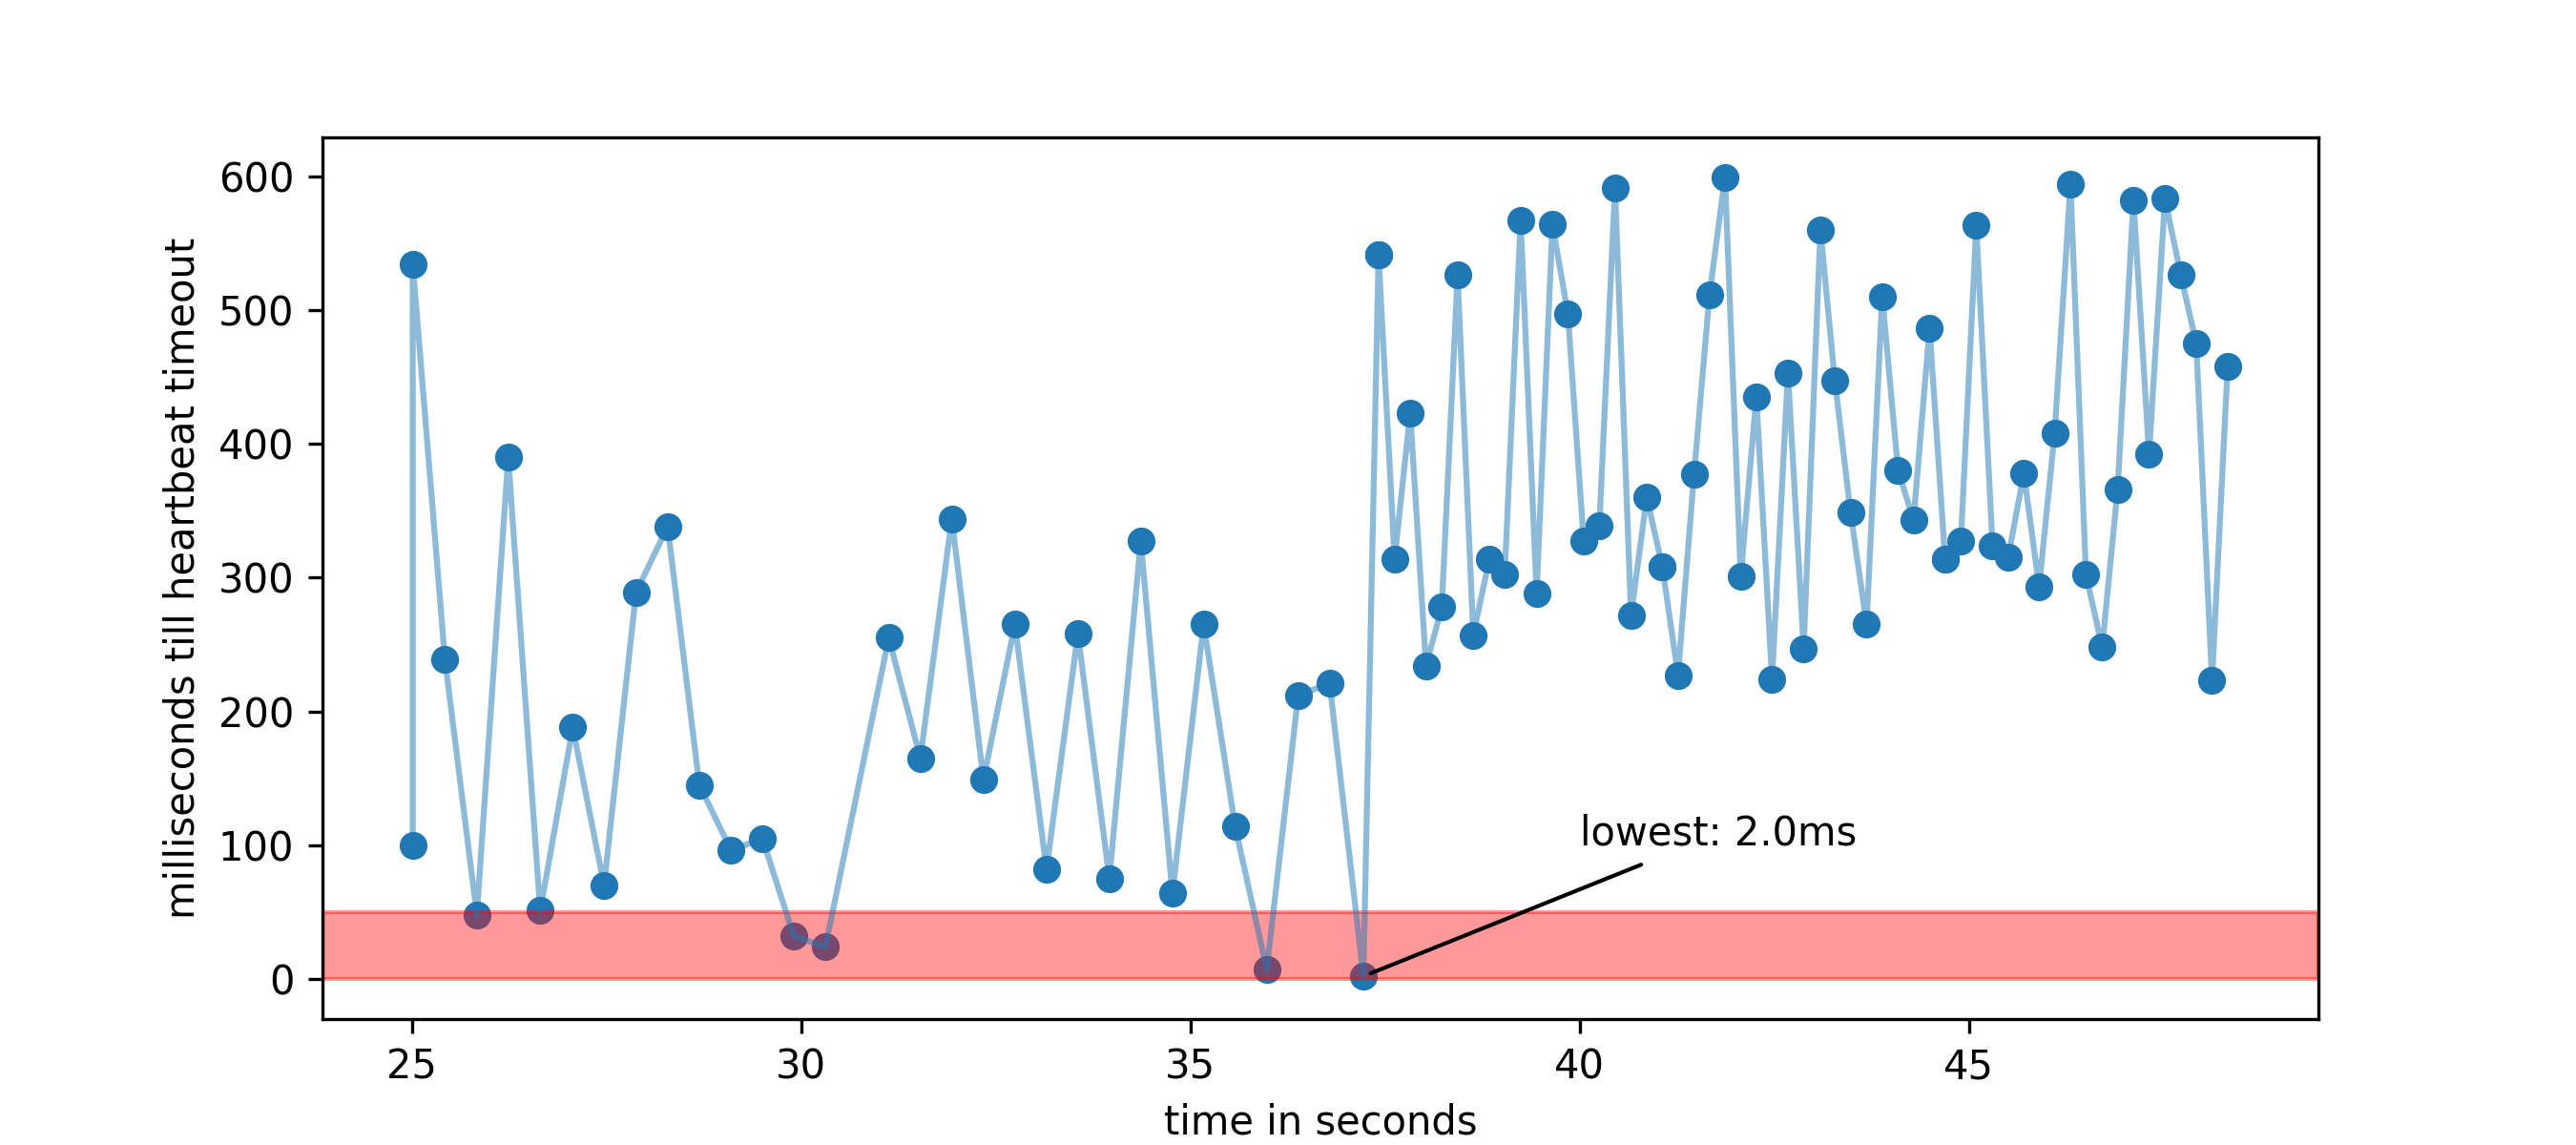
\includegraphics{../data/hb_timeout.png}
	\caption{Time left before the the heartbeat times out while recieving sequential make directory requests. Around 37 seconds the writeserver timed out and a new writeserver took over because an other readserver timed out. Unencomburd by the mkdir requests the new writeservers heartbeat arive well on time.}
	\label{fig:hbt}
\end{figure}
